\documentclass[11pt]{article}

\usepackage[a4paper,margin=25mm,headheight=15pt]{geometry}
\usepackage[T1]{fontenc}
\usepackage[utf8]{inputenc}
\usepackage{lmodern}
\usepackage{microtype}
\usepackage{amsmath}
\usepackage{booktabs}
\usepackage{array}
\usepackage{longtable}
\usepackage{enumitem}
\usepackage{xcolor}
\usepackage{fancyhdr}
\usepackage{tikz}
\usetikzlibrary{arrows.meta,positioning,shapes.geometric}
\usepackage[hidelinks]{hyperref}

\definecolor{Accent}{HTML}{315B7D}
\definecolor{NoteBlue}{HTML}{EAF2F8}
\definecolor{NoteBorder}{HTML}{7BA5C4}
\definecolor{Muted}{HTML}{5B6570}

\hypersetup{
  pdftitle={Materials and Methods (Module 0, _PK): LD decay and LD-based complexity reduction},
  pdfauthor={Poikela et al.},
  pdfsubject={Hybrid genome evolution in Formica wood ants}
}

\pagestyle{fancy}
\fancyhf{}
\lhead{\small\color{Muted}Materials and Methods (Module 0)}
\rhead{\small\color{Muted}Poikela et al.}
\cfoot{\small\thepage}
\renewcommand{\headrulewidth}{0.4pt}

\setlength{\parindent}{0pt}
\setlength{\parskip}{0.65em}
\setlist[itemize]{leftmargin=1.5em,itemsep=0.2em,topsep=0.25em}
\setlist[enumerate]{leftmargin=1.7em,itemsep=0.25em,topsep=0.25em}
\renewcommand{\arraystretch}{1.15}
\renewcommand{\thesection}{S\arabic{section}}
\renewcommand{\thesubsection}{\thesection.\arabic{subsection}}

\newcommand{\Faq}{\textit{F.~aquilonia}}
\newcommand{\Fpo}{\textit{F.~polyctena}}
\newcommand{\rsq}{\ensuremath{r^{2}}}
\newcommand{\todo}[1]{%
  \par\noindent
  \fcolorbox{NoteBorder}{NoteBlue}{%
    \parbox{\dimexpr\linewidth-2\fboxsep-2\fboxrule\relax}{%
      \textbf{Open item.} #1}}%
  \par}

\title{\vspace{-3em}
  \textbf{\color{Accent}Materials and Methods}\\[0.3em]
  \Large LD decay and LD-based complexity reduction}
\author{Poikela et al.}
\date{\small Module 0 (\texttt{\_PK} pipeline)}

\begin{document}
\maketitle
\vspace{-1.5em}

\begin{center}
\small\color{Muted}
Working draft for the \texttt{\_PK} pipeline. It covers marker processing, LD
decay and per-marker local LD support, and the two-stage LD-based complexity
reduction that yields the shared LD-reduced units. Ancestry sorting and genomic
architecture, which use these units, are documented in the Module~A methods.
Blue boxes mark items that remain open.
\end{center}

\section{Scope and analytical principles}

These methods describe LD decay estimation and LD-based complexity reduction,
which transform the marker data into the shared set of LD-reduced analytical
units used by the downstream ancestry-sorting and genomic-architecture analyses
(Module~A).

Three principles guided the analyses. First, markers in LD carry partly
redundant information. We therefore used clusters of strongly correlated
markers as LD-reduced analytical units wherever possible, while retaining
marker-level analyses as diagnostics of spatial pseudoreplication. We do not
assume that the resulting units are strictly statistically independent.
Second, a variable evaluated as a predictor was not also used to select the
analysed data. In particular, loci were gated by parental allele frequency
rather than by the diagnostic index (DI), leaving the full range of DI
available for analysis. Third, these analyses do not assume complete demographic
independence of the twenty hybrid populations; analyses that use variation among
populations are interpreted as descriptive associations.

\todo{The general sample description currently reports 165 sequenced hybrid
individuals, whereas the analysis objects contain 164. Confirm which individual
was excluded, most likely because of excessive missing data, and report the
identifier and exclusion criterion in the final text. Until then, 164 is used
for all analysis-specific counts.}

\begin{figure}[htbp]
\centering
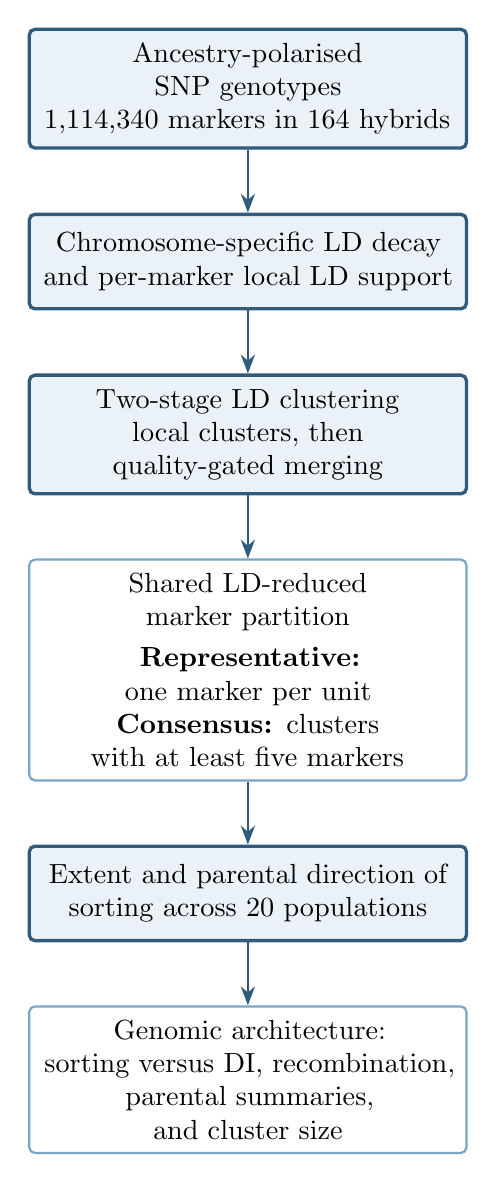
\begin{tikzpicture}[
  node distance=8mm and 12mm,
  box/.style={
    draw=Accent, rounded corners=2pt, very thick, fill=NoteBlue,
    align=center, text width=52mm, minimum height=12mm, inner sep=5pt
  },
  result/.style={
    draw=NoteBorder, rounded corners=2pt, thick, fill=white,
    align=center, text width=52mm, minimum height=12mm, inner sep=5pt
  },
  arrow/.style={-{Stealth[length=2.4mm]}, thick, draw=Accent}
]
\node[box] (genotypes) {Ancestry-polarised SNP genotypes\\
1,114,340 markers in 164 hybrids};
\node[box, below=of genotypes] (ld) {Chromosome-specific LD decay\\
and per-marker local LD support};
\node[box, below=of ld] (cluster) {Two-stage LD clustering\\
local clusters, then quality-gated merging};
\node[result, below=of cluster] (projections)
{Shared LD-reduced marker partition\\[1mm]
\textbf{Representative:} one marker per unit\\
\textbf{Consensus:} clusters with at least five markers};
\node[box, below=of projections] (sorting)
{Extent and parental direction of\\ sorting across 20 populations};
\node[result, below=of sorting] (architecture) {Genomic architecture:\\
sorting versus DI, recombination,\\ parental summaries, and cluster size};

\draw[arrow] (genotypes) -- (ld);
\draw[arrow] (ld) -- (cluster);
\draw[arrow] (cluster) -- (projections);
\draw[arrow] (projections) -- (sorting);
\draw[arrow] (sorting) -- (architecture);
\end{tikzpicture}
\caption{\textbf{Analytical workflow.} LD decay and clustering
transform the marker data into a shared set of LD-reduced units represented
either by a single marker or, for larger clusters, by a consensus genotype. The
same units feed the analyses of the extent, direction and genomic architecture
of ancestry sorting.}
\label{fig:workflow}
\end{figure}

\subsection{Marker processing and ancestry orientation}

Genotypes and marker-level ancestry information were obtained from the DIEM
output for this data set. Sites were restricted to biallelic markers. DIEM
provides a polarity and a diagnostic index for each marker. The diagnostic
index measures the degree to which allele frequencies differentiate the
parental reference samples. For markers with the opposite polarity, genotype
dosages were replaced by \(2-\mathrm{dosage}\), placing dosages on a consistent
ancestry-oriented scale across the genome.

Minor allele frequency (MAF) was calculated among hybrid individuals only, and
markers with hybrid MAF \(\geq 0.05\) were retained. The resulting analysis set
contained 1,114,340 markers. Two matrices were constructed over this same
marker set. The hybrids-only matrix was used for LD estimation, clustering, and
complexity reduction. A second matrix containing hybrids and parental
references was used when parental allele frequencies were required, including
ancestry orientation and marker-level parental summaries. Keeping the parents
out of the LD calculations prevents parent--hybrid differentiation from dominating
estimates intended to describe LD within the hybrid populations.

\section{LD decay and local LD support}

\subsection{Chromosome-specific LD decay}

LD decay was modelled separately for each chromosome as
\begin{equation}
  r^2(d) = b + \frac{c-b}{1+a d},
  \label{eq:lddecay}
\end{equation}
where \(d\) is physical distance in base pairs, \(a\) is the decay rate,
\(b\) is long-range background \(r^2\), and \(c\) is short-range \(r^2\).
Background LD was estimated from inter-chromosomal marker pairs. Within each
chromosome, the curve was fitted across twenty sliding windows with 50\%
overlap. Up to 5,000 marker pairs were sampled per window, stratified across
twenty distance classes to represent short and long distances comparably.

Within each distance class, LD was summarized by the \(0.95\) quantile of \(r^2\) to characterize the upper LD landscape, which was the primary interest of this analysis. Parameter estimates were subsequently aggregated over the central 95\% of windows to limit the influence of extreme outlier window-level fits (LD-decay supplementary figure).

Only pairs for which both markers had MAF \(>0.1\) contributed to the
background and decay-curve fits. This restriction reduces the frequency-driven
depression of \(r^2\) at rare alleles.

Since crossover number generally scales less than proportionally with physical chromosome length, this predicts  greater recombination per unit physical distance, and consequently faster LD decay, on shorter chromosomes. A robust regression of \(a\) on
chromosome size was therefore fitted genome-wide. For a relative decay threshold \(\rho\), defined as the proportion of the fitted short-distance LD that had decayed, the corresponding physical distance was calculated as
\begin{equation}
  d = \frac{\rho}{a(1-\rho)}.
  \label{eq:distance}
\end{equation}
 This allowed window sizes to reflect each chromosome's fitted decay behaviour rather than imposing a single physical-distance threshold across the genome.

\subsection{Per-marker local LD support}

For each marker, local LD support (\(\mathrm{ld}_w\)) was calculated as the
median \(r^2\) between that marker and neighbouring markers within the window
corresponding to \(\rho=0.95\) that denotes the distance at which LD has declined by 95\% relative to its fitted short-distance value. Unlike map-based recombination rate, \(\mathrm{ld}_w\) is measured directly from the genotype data at marker resolution and requires no interpolation.

We evaluated \(\mathrm{ld}_w\) and the window-level decay rate \(a\) as
indicators of low recombination using map-based recombination rate as a
reference. Across definitions based on the lowest 5\%, 10\%, and 25\% of
recombination windows, the area under the receiver-operating-characteristic
curve was 0.91--0.98 for \(a\) and 0.73--0.86 for \(\mathrm{ld}_w\).
Accordingly, \(a\) was the stronger window-level indicator, whereas
\(\mathrm{ld}_w\) supplied the marker-resolution measure needed to identify
clusters for reconsideration during complexity reduction
(the recombination-discrimination and local-LD-track supplementary figures).

\section{Two-stage LD-based complexity reduction}

\subsection{Terminology and outputs}

The procedure has two stages: (i) local clustering with a complete-linkage
refinement and (ii) targeted, quality-gated merging. Both stages define a single
partition of markers, from which two representations are produced:
\begin{itemize}
  \item one representative marker per cluster, forming an LD-pruned marker set;
  \item one expected multi-locus genotype (eMLG) consensus dosage for clusters
        containing at least five markers.
\end{itemize}

We use ``LD cluster'' or ``LD-reduced unit'' for a set of strongly correlated
markers. These units are not haplotype blocks: markers are grouped by the
partition of sampled chromosomes that they report, and clusters may therefore
overlap in physical position. The procedure reduces redundancy and constrains residual LD but does not make them strictly independent; the remaining
dependence is assessed or controlled where it matters downstream.

\subsection{Stage 1: local clustering}

For each chromosome, the clustering distance was derived from its fitted LD
decay curve at the half-way decay distance \(\rho=0.5\). The threshold was not allowed to vary further
within chromosomes, because locally elevated LD is precisely where redundant
markers should be grouped more strongly.

Clustering was performed on a sparse LD graph constructed from pairwise LD estimates between markers separated by no more than 400 SNPs, a neighborhood spanning approximately the $\rho=0.99$ decay distance. Markers were first
assigned to connected components of the thresholded graph (single linkage clustering). Each component was
then refined by complete-linkage hierarchical clustering using the dense
pairwise \(r^2\) matrix within the component. The complete-linkage step limits
single-linkage chaining, in which two weakly correlated markers could otherwise
be joined through an intermediate marker correlated with both. The representative marker of a cluster was the member with the highest median
\(r^2\) to the other cluster members.

\subsection{Stage 2: targeted, quality-gated merging}

The finite window used to construct the Stage 1 edge list makes the first stage
conservative in extended low-recombination regions: marker pairs outside the
window are not evaluated and therefore cannot satisfy complete linkage. Stage
2 reconsidered candidate clusters directly from their genotypes, without the
Stage 1 window restriction.

A Stage 1 cluster was carried forward as a candidate for Stage 2 merging if any member had \(\mathrm{ld}_w>0.025\) or if the cluster contained at least five markers. This screening reduced unnecessary graph comparisons: small clusters composed entirely of low-\(\mathrm{ld}_w\) markers were unlikely to show sufficient LD with neighbouring clusters to merge and were therefore left unchanged. The size criterion nevertheless retained larger Stage 1 clusters for evaluation even when none of their individual markers exceeded the local-LD threshold.

Flagged clusters were considered for merging using a distance-restricted,
average-linkage dynamic tree cut. A candidate merge was accepted only while
both of the following criteria were satisfied:
\begin{enumerate}
  \item consensus fidelity
  \[
    \mathrm{score}_{\mathrm{eMLG}}(x)
    =\mathrm{cor}\{\mathrm{round}(x),x\}^{2} \geq 0.80;
  \]
  \item a pairwise correlation floor of \(r^2\geq0.2\) between the sides being
        merged.
\end{enumerate}

The fidelity criterion evaluates whether the resulting consensus remains close
to a discrete genotype. The correlation floor prevents a small, weakly related
set of markers from being absorbed into a large cluster whose existing
consensus would otherwise dominate the fidelity score. These gates constrain
merging but do not establish complete statistical independence among the final
units. Observed residual correlations among neighbouring merged units were of
order \(r^2\approx0.3\) after correction for relatedness and were local in
genetic distance.

Candidate merges were restricted to clusters separated by no more than 1.0~cM on the genetic map so that the resulting units primarily represented local linkage. Persistent LD across greater recombinational distances is less readily attributable to limited recombination alone and may instead reflect processes such as population structure, admixture history or selection. Such long-range associations were therefore retained as relationships between distinct units rather than used to collapse them into a single cluster.

\subsection{Output and validation}

The final partition contained 470,035 LD clusters. Of these, 32,871 contained
at least five markers and had an eMLG consensus. Smaller
clusters remain valid LD-reduced units and retain their representative marker;
the five-marker threshold is therefore a threshold for storing a consensus,
not for defining a cluster.

The procedure was evaluated by comparing Stage 1 and combined Stage 1--2
clusterings in extended-LD regions (Stage-1-versus-combined supplementary figure), by examining the
distribution of consensus fidelity across \(\mathrm{ld}_w\) thresholds
(consensus-fidelity supplementary figure), and by quantifying the ability of
\(\mathrm{ld}_w\) to identify low-recombination regions. These checks assess
whether Stage 2 consolidates fragmentation where long-range LD is present
without broadly collapsing weakly correlated markers.


\section{Software, reproducibility, and current status}

LD decay estimation, clustering, and consensus construction were implemented
using functions from \texttt{LDscnR}. Project-level analyses were performed in R
using scripts in the \texttt{formica\_hybrid} repository, folder
\texttt{module0\_ld\_pruning/R/}: \texttt{module0\_LD\_decay\_from\_DIEM.R} (LD
decay and per-marker local LD support), \texttt{module0\_ld\_pruning\_DIEM.R}
(two-stage clustering and consensus construction), and
\texttt{module0\_fig\_ld\_tracks.R} (local-LD track figures). Shared genotype
inputs are read from \texttt{data/}; module-specific intermediates and the final
clustering are written to \texttt{module0\_ld\_pruning/data/}; figures to
\texttt{module0\_ld\_pruning/Figures/}.

\todo{Add the final \texttt{LDscnR} citation, version, and repository or archive
identifier before submission.}

\begin{longtable}{>{\raggedright\arraybackslash}p{0.20\textwidth}
                  >{\raggedright\arraybackslash}p{0.42\textwidth}
                  >{\raggedright\arraybackslash}p{0.27\textwidth}}
\caption{Principal parameter settings (Module 0).}
\label{tab:parameters0}\\
\toprule
Analysis & Parameter & Value \\
\midrule
\endfirsthead
\toprule
Analysis & Parameter & Value \\
\midrule
\endhead
Marker set & Hybrid MAF threshold & \(\geq0.05\) \\
           & Retained markers & 1,114,340 \\
\midrule
LD decay & Windows per chromosome & 20, 50\% overlap \\
         & Marker pairs per window & \(\leq5,000\), 20 distance strata \\
         & \(r^2\) summary & 0.95 quantile \\
         & Pair MAF for curve fitting & \(>0.1\) for both members \\
\midrule
Stage 1 & Relative LD threshold & \(\rho=0.5\), per chromosome \\
        & Clustering & connected components, then complete linkage \\
        & Representative & highest median \(r^2\) to cluster members \\
\midrule
Stage 2 & Flagging & \(\mathrm{ld}_w>0.025\) or \(\geq5\) markers \\
        & Consensus fidelity & \(\geq0.80\) \\
        & Pairwise correlation floor & \(r^2\geq0.2\) \\
        & Distance restriction & 1.0 cM \\
        & Stored consensus & clusters with \(\geq5\) markers \\
        & Final partition & 470,035 clusters; 32,871 with consensus \\
\bottomrule
\end{longtable}

\end{document}
